\documentclass[12pt]{article}

% UTF-8 encoding and fonts
\usepackage[utf8]{inputenc}
\usepackage[T1]{fontenc}
\usepackage{lmodern}

% Page setup
\usepackage[margin=1in]{geometry}
\usepackage{setspace}
\onehalfspacing

% Typography
\usepackage{microtype}

% Math and symbols
\usepackage{amsmath,amssymb}

% Graphics
\usepackage{graphicx}
\usepackage{float}
\usepackage{subcaption}

% Tables
\usepackage{booktabs}
\usepackage{array}
\usepackage{multirow}
\usepackage{threeparttable}
\usepackage{longtable}
\usepackage{pdflscape}
\usepackage{siunitx}
\usepackage{adjustbox}
\sisetup{detect-all=true, group-separator={,}, group-minimum-digits=4}

% Bibliography
\usepackage{natbib}
\bibliographystyle{aer}

% Hyperlinks
\usepackage{hyperref}
\hypersetup{
    colorlinks=true,
    linkcolor=blue,
    citecolor=blue,
    urlcolor=blue
}
\usepackage[nameinlink,noabbrev]{cleveref}

% Timing data
\IfFileExists{timing_data.tex}{\input{timing_data.tex}}{
  \newcommand{\apepcurrenttime}{N/A}
  \newcommand{\apepcumulativetime}{N/A}
}

% Captions
\usepackage{caption}
\captionsetup{font=small,labelfont=bf}

% Section formatting
\usepackage{titlesec}
\titleformat{\section}{\large\bfseries}{\thesection.}{0.5em}{}
\titleformat{\subsection}{\normalsize\bfseries}{\thesubsection}{0.5em}{}

% Custom commands
\newcommand{\E}{\mathbb{E}}
\newcommand{\Var}{\text{Var}}
\newcommand{\Cov}{\text{Cov}}
\newcommand{\ind}{\mathbb{I}}
\newcommand{\sym}[1]{\ifmmode^{#1}\else\(^{#1}\)\fi}

\title{The Decade of Decline: How the Austerity Pay Squeeze on Teachers Shaped Student Achievement in England}
\author{APEP Autonomous Research\thanks{Autonomous Policy Evaluation Project. Correspondence: scl@econ.uzh.ch{} (cumulative: \apepcumulativetime{}).} \and @SocialCatalystLab}
\date{\today}

\begin{document}

\maketitle

\begin{abstract}
\noindent
In 2010, the typical English teacher earned 25 percent more than the local private-sector median. By 2019, after a decade of pay restraint, that premium had vanished in high-cost areas while persisting in low-wage regions. This paper uses the divergence between frozen national teacher pay and rising local private wages to examine whether teacher pay competitiveness affects student achievement. Using doubly robust estimation, I find that local authorities where pay competitiveness eroded most scored 1.12 Attainment~8 points lower---roughly one-third of a cross-LA standard deviation ($p=0.037$ in-sample, though cross-fitted inference is insignificant). The association survives omitted variable diagnostics (Oster $\delta=2.1$) but is sensitive to region composition and a placebo test. These findings are suggestive of an achievement cost to pay erosion, though data limitations prevent a definitive causal interpretation.
\end{abstract}

\vspace{1em}
\noindent\textbf{JEL Codes:} I21, J31, J45, H52 \\
\noindent\textbf{Keywords:} teacher pay, austerity, student achievement, doubly robust estimation, England

\newpage

%=============================================================================
\section{Introduction}
%=============================================================================

In 2010, a mid-career teacher in England earned \textsterling{}14.15 an hour---25 percent above the local private-sector median in a typical local authority. A decade later, after the longest public-sector pay freeze in modern British history, that premium had shrunk to single digits nationally and vanished entirely in parts of London and the South East. The midpoint of the teacher pay scale rose just 4 percent in nominal terms between 2010 and 2019---less than half the rate of inflation---while median private-sector earnings grew by over 20 percent.

This paper asks whether that erosion of teacher pay competitiveness affected student achievement. The question matters for two reasons. First, teacher quality is the single most important school-level determinant of student outcomes \citep{rivkin2005teachers, chetty2014measuring1, chetty2014measuring2, hanushek2011economic}. Second, the mechanism linking pay to outcomes---through recruitment, retention, and effort---is central to education policy debates worldwide, yet causal evidence from real-world pay changes remains sparse \citep{dolton2011if, britton2016teacher}.

I exploit a natural feature of England's institutional setting: the School Teachers' Pay and Conditions Document (STPCD) sets a national pay scale that binds across most state-funded schools, while private-sector wages vary substantially across local labour markets \citep{allen2018understanding}. The austerity-era freeze therefore created differential ``competitiveness shocks'' across local authorities (LAs). In areas where private-sector wages grew fastest---primarily London and the South East---teacher pay became relatively less attractive. In areas where private-sector wages also stagnated---typically post-industrial areas in the North and Midlands---teachers' relative position was more insulated. This geographic variation in the \textit{change} in the teacher-to-private pay ratio between 2010 and 2019 provides the identifying variation.

I measure competitiveness as the ratio of the STPCD midpoint salary to the local median private-sector annual pay from the Annual Survey of Hours and Earnings (ASHE). I define treatment as belonging to the bottom quartile of the competitiveness change distribution---the 36 local authorities where the ratio declined most sharply. The primary outcomes are Attainment~8 scores from Key Stage~4 GCSE results in the post-austerity years (2021/22--2023/24), which I link to the pre-determined treatment exposure.

The econometric challenge is that the competitiveness decline is not randomly assigned. Local authorities where teacher pay became least competitive tend to have higher baseline private-sector wages and are disproportionately located in London and the South East---areas that also differ in school quality, demographics, and education spending. To address this, I employ doubly robust augmented inverse probability weighting (DR-AIPW), following \citet{robins1994estimation}, which combines a propensity score model for treatment assignment with an outcome regression model. The estimator is consistent if either the propensity score or the outcome model is correctly specified \citep{heckman1998characterizing}.

The in-sample doubly robust estimator with Random Forest nuisance functions yields a point estimate of $-1.12$ Attainment~8 points ($p = 0.037$), roughly one-third of a cross-LA standard deviation---equivalent to about one grade in one GCSE subject. However, a cross-fitted implementation (which guards against overfitting) produces a wider confidence interval that includes zero. Parametric and continuous dose-response specifications point in the same direction, with each unit increase in the competitiveness ratio predicting 7.7 higher Attainment~8 points ($p = 0.049$).

Several diagnostic tests inform the interpretation. Oster's (2019) coefficient stability test yields $\delta = 2.13$, suggesting that unobservable confounders would need to be more than twice as important as the observed covariates to explain away the result. The E-value of 1.92 quantifies the required strength of unmeasured confounding \citep{vanderweele2017sensitivity}. However, three results counsel caution. First, randomization inference provides an exact $p$-value of 0.236 for the OLS specification, and cross-fitted inference with out-of-fold nuisance estimation is insignificant. Second, the result is fragile to the exclusion of Unitary authorities, which constitute the majority of treated units. Third---and most concerning---a placebo test using 2005--2010 competitiveness changes yields a coefficient of similar magnitude ($-1.12$, $p = 0.101$), suggesting that persistent structural differences between high- and low-wage-growth areas may drive the association. These findings are consistent with a causal effect of pay erosion on achievement, but cannot definitively rule out confounding from the local economic conditions that simultaneously generated the competitiveness variation.

I find no evidence that the competitiveness shock widened the free school meals (FSM) achievement gap. The treatment effect on the within-LA gap between FSM and non-FSM students is effectively zero ($0.07$, $p = 0.913$). If the mechanism operates through teacher supply rather than within-school sorting, this null is consistent with a compositional channel: areas losing relative pay attract fewer entrants across the board, rather than selectively losing teachers from disadvantaged schools.

This paper contributes to several literatures. First, it adds to the literature on teacher pay and student achievement. While cross-country evidence links teacher compensation to outcomes \citep{dolton2011if}, within-country causal estimates are rare. \citet{hendricks2014relative} exploits variation in the teacher wage premium across Florida counties, finding significant effects on student test scores. \citet{britton2016teacher} study English academy schools that gained freedom to set their own pay, finding that schools in competitive labour markets used this flexibility. I complement these studies by examining a system-wide pay shock that affected all state schools simultaneously.

Second, the paper contributes to the literature on the effects of fiscal austerity on public services. The UK's post-2010 consolidation reduced real public spending per capita by over 10 percent, with effects documented across health \citep{nickell2005poverty}, policing, and local government. Education has received less attention despite being one of the largest items of public expenditure. \citet{sims2020teacher} documents the effect of pay restraint on teacher supply in England, finding a significant negative impact on applications; I extend this line by estimating downstream effects on achievement.

Third, the identification strategy---exploiting the interaction between nationally uniform pay and spatially heterogeneous outside options---has methodological implications for evaluating centralized pay systems. \citet{allen2018understanding} provide descriptive evidence of this interaction, and the School Teachers' Review Body has repeatedly flagged geographic recruitment challenges \citep{strb2023report}. My estimates provide a causal framework for quantifying the achievement costs.

The remainder of the paper is organized as follows. Section~\ref{sec:background} describes the institutional setting. Section~\ref{sec:framework} outlines the conceptual framework. Section~\ref{sec:data} describes the data sources. Section~\ref{sec:strategy} presents the empirical strategy. Section~\ref{sec:results} reports the results, including robustness and sensitivity analyses. Section~\ref{sec:discussion} discusses interpretation and limitations. Section~\ref{sec:conclusion} concludes.


%=============================================================================
\section{Institutional Background}\label{sec:background}
%=============================================================================

\subsection{The Teacher Pay System in England}

Teacher pay in England's state-funded schools is governed by the School Teachers' Pay and Conditions Document (STPCD), published annually by the Department for Education following recommendations from the independent School Teachers' Review Body (STRB). The STPCD defines a main pay range with six reference points (M1 through M6) and an upper pay range with three points, along with separate scales for leadership. Since 2004, the system has distinguished four geographical pay bands: Inner London, Outer London, the ``London Fringe'' (surrounding counties), and the ``Rest of England,'' reflecting the higher cost of living in and around the capital.

Two features of this system are central to the identification strategy. First, the STPCD is \textit{binding} for maintained schools, which must set pay within the statutory ranges. While academies---state-funded schools operating outside local authority control---are technically free to set their own pay, \citet{britton2016teacher} show that the vast majority continue to follow STPCD scales. Thus, for practical purposes, teacher pay is set nationally and varies across space only through the London weighting bands.

Second, the STPCD determines \textit{nominal} pay levels, not real or relative ones. When the government freezes the statutory scale, teachers' real pay falls with inflation, and their relative pay falls further if private-sector wages grow. The extent of this relative decline depends entirely on local labour market conditions: in areas where alternative wages grow rapidly, the teaching profession becomes relatively less attractive; in areas where alternative wages stagnate, the freeze has minimal competitive effect.

\subsection{The Austerity Pay Freeze (2010--2019)}

Following the 2010 Comprehensive Spending Review, the Coalition government announced a two-year pay freeze for all public-sector workers earning above \textsterling{} 21,000, followed by a 1 percent annual cap on pay increases. For teachers, this translated into minimal nominal growth in STPCD reference points between 2010 and 2016 (\Cref{tab:stpcd}): a two-year freeze followed by four years of 1 percent annual increases. The M1 starting salary for the Rest of England stood at \textsterling{} 21,588 in 2010 and had risen only to \textsterling{} 22,467 by 2016---a cumulative increase of 4 percent against CPI inflation of approximately 15 percent, representing a real-terms pay cut of over 10 percent.

From 2017 to 2019, the cap was nominally lifted but pay awards remained modest (1--3.5 percent). Only after the 2022 STRB report did starting salaries receive substantial increases, reaching \textsterling{} 30,000 by 2023. However, by this point, teachers had experienced nearly a decade of real pay erosion.

The freeze affected all state-funded teachers equally in nominal terms. But because local private-sector labour markets diverged substantially during this period---with strong wage growth in London, the South East, and technology hubs, versus weak growth in deindustrialized areas---the \textit{competitive} impact was spatially heterogeneous. This heterogeneity is the source of identifying variation.

\subsection{Local Authority Geography}

England's education governance structure involves several types of local authority. Upper-tier authorities---counties (E10 codes), metropolitan boroughs (E08), unitary authorities (E06), and London boroughs (E09)---are responsible for education services including school place planning, special educational needs provision, and, for maintained schools, admissions and funding allocation. Lower-tier district councils (E07) nest within county councils and have no direct education responsibilities.

The ASHE earnings data are reported at the district level, which does not align with education authority boundaries. I address this by aggregating district-level earnings within county boundaries using an explicit lookup table, and combining these with direct observations for unitary authorities, metropolitan boroughs, and London boroughs. This yields 146 education-authority-aligned local authorities with both earnings and achievement data.

\subsection{The Academisation Programme and Pay Freedom}

A complication for the identification strategy is the rapid expansion of academies since 2010. The Academies Act 2010 accelerated conversion of maintained schools to academy status, and by 2019 approximately 75 percent of secondary schools were academies. Academies are formally exempt from STPCD pay requirements and can set their own salary structures.

In practice, however, the vast majority of academies continue to follow STPCD scales or closely mirror them. \citet{britton2016teacher} find that only a small minority of academy trusts---typically large multi-academy trusts operating in competitive urban labour markets---exercise meaningful pay freedom. The median academy pays within 2 percent of the STPCD scale. This means the national pay freeze effectively bound most academy schools as well, preserving the validity of using the STPCD midpoint as the relevant teacher salary across all state-funded schools.

The regional concentration of pay-flexible academies---disproportionately located in London and the South East---introduces a potential confound: areas where private wages grew fastest (eroding competitiveness) may also be areas where some academies used pay freedom to counteract the freeze. This would attenuate the estimated effect, biasing results toward zero. The estimates should therefore be interpreted as lower bounds on the competitiveness effect, since some treated areas may have partially offset the squeeze through academy pay flexibility.

\subsection{Teacher Supply During Austerity}

The aggregate evidence on teacher supply during the freeze period provides important context for interpreting the achievement results. Initial teacher training (ITT) recruitment fell below target in most years between 2012 and 2019, with the shortfall most acute in mathematics, physics, and computing \citep{allen2018teacher, epi2019teacher}. The teacher vacancy rate, which the School Workforce Census measures as the proportion of posts advertised but unfilled at the November census date, rose from 0.1 percent in 2010 to 0.4 percent by 2018---a quadrupling that, while small in absolute terms, represents thousands of classrooms.

\citet{sims2020teacher} provides the most rigorous analysis of the pay-supply link. Using variation in the real value of the teacher pay premium across regions and time, he estimates that a 10 percent reduction in the pay premium reduces applications to ITT by 11--13 percent, with a long-run elasticity of approximately 1.3. The effect is larger for STEM subjects and for male applicants, who face better outside options in the private sector.

Retention data tell a similar story. The ``leaving rate'' for qualified teachers in state-funded schools rose from 9.2 percent in 2010 to 10.6 percent by 2019, with the increase concentrated among teachers in their first five years \citep{ifs2019teacher}. Early-career attrition is particularly costly because it squanders the public investment in training and removes teachers before they reach peak effectiveness (typically around years 5--10 of experience).

These supply-side trends are the plausible mechanisms linking competitiveness erosion to achievement. A local authority where the teaching profession became less attractive relative to alternatives would experience both fewer new entrants and higher attrition. Over the course of a decade, these flows would compound into a measurably less experienced, and potentially lower-quality, teaching workforce.

%=============================================================================
\section{Conceptual Framework}\label{sec:framework}
%=============================================================================

I model the relationship between teacher pay competitiveness and student achievement through a simple labour market framework. Let $w_j^T$ denote the teacher salary in local authority $j$ (set by STPCD) and $w_j^P$ the median private-sector wage. The competitiveness ratio is:
\begin{equation}
R_j = \frac{w_j^T}{w_j^P}
\end{equation}

A potential teacher in area $j$ compares teaching against outside options. The probability of entering (or remaining in) teaching is:
\begin{equation}
\Pr(\text{teach}_j) = f(R_j, \mathbf{X}_j)
\end{equation}
where $\mathbf{X}_j$ captures non-pecuniary factors (working conditions, prestige, intrinsic motivation). When the pay freeze holds $w_j^T$ constant while $w_j^P$ grows, $R_j$ falls. The decline is larger in areas where private wages grow faster, creating spatial variation in the teaching profession's attractiveness.

The link to student achievement operates through three channels. \textit{Recruitment}: lower $R_j$ reduces the pool of applicants and lowers the average quality of new entrants \citep{hanushek2011economic}. \textit{Retention}: experienced teachers facing better outside options are more likely to leave, reducing average teacher experience \citep{gilpin2011reevaluating, imazeki2005does}. \textit{Effort}: teachers who feel underpaid may reduce discretionary effort, though this channel is harder to measure \citep{jackson2018does}.

The key testable prediction is:
\begin{equation}
\frac{\partial Y_j}{\partial R_j} > 0
\end{equation}
where $Y_j$ is average student achievement in area $j$. Areas experiencing larger declines in $R_j$ during the austerity period should exhibit lower post-austerity achievement, conditional on baseline characteristics.

An important nuance is timing. The pay freeze began in 2010, but its effects on student achievement operate with a lag: it takes time for recruitment and retention changes to alter the teacher workforce composition, and for workforce changes to affect the cohort of students sitting GCSEs. The post-COVID exam cohorts (2021/22 onwards) took their GCSEs approximately 5--10 years into the freeze, which should capture medium-run effects through the recruitment and retention channels.

%=============================================================================
\section{Data}\label{sec:data}
%=============================================================================

\subsection{Annual Survey of Hours and Earnings (ASHE)}

Private-sector wages come from the Annual Survey of Hours and Earnings, accessed via the NOMIS API (dataset NM\_99\_1). ASHE is a 1 percent sample of employees linked to HM Revenue and Customs records, providing median gross annual pay by local authority district for all employees regardless of industry. I extract data for 2005--2023 covering all English local authority districts (TYPE464 geography), filtering to the median (item 2) of annual gross pay (pay code 7) for all employees (sex code 7).

ASHE reports at the district level. For the 21 two-tier counties (E10 codes) where education responsibilities sit at the county level, I aggregate district earnings by computing the unweighted mean of constituent district medians. This yields 146 education-authority-aligned observations per year: 25 unitary authorities with E06 codes, 36 metropolitan boroughs (E08), 32 London boroughs (E09), 21 aggregated counties (E10), and additional authorities with other codes.

\subsection{Key Stage 4 GCSE Results}

Student achievement data come from the Department for Education's Explore Education Statistics service, accessed via the public API. The Key Stage 4 dataset provides local-authority-level GCSE results including Attainment~8, Progress~8, and English and Mathematics basics pass rates. Data are available at the local authority level from the 2018/19 academic year onward.

Attainment~8 measures each student's performance across eight GCSE subjects, with a maximum possible score of 90. It was introduced in 2016 and is the primary headline accountability measure. Progress~8 adjusts for prior attainment at Key Stage~2, providing a value-added measure. I also extract outcomes stratified by free school meals (FSM) eligibility to compute within-LA achievement gaps.

I drop the 2019/20 and 2020/21 academic years because GCSE exams were cancelled due to COVID-19 and replaced with teacher-assessed or centre-assessed grades. The analysis sample therefore covers 2018/19 (pre-COVID) and 2021/22 through 2023/24 (post-COVID).

\subsection{Teacher Pay Scales (STPCD)}

I construct teacher pay series from published STPCD documents (2005--2023), recording the M1 (starting salary) and M6 (top of main range) reference points for the Rest of England pay band. The midpoint, $(M1 + M6)/2$, serves as the typical teacher salary used in the competitiveness ratio. Table~\ref{tab:stpcd} in the Appendix reports the full series.

\subsection{Sample Construction and Key Variables}

The analysis panel merges ASHE earnings, KS4 outcomes, and STPCD pay scales at the local-authority-by-year level. The backbone of the panel is the ASHE earnings data, which provides 146 education-authority-aligned observations per year from 2005 to 2023 (2,680 total LA-year observations). STPCD pay scales are year-specific (not geography-specific within the Rest of England band), so the merge is one-to-many: each year's STPCD midpoint is matched to all local authorities.

\textbf{Calendar-year to academic-year alignment.} ASHE reports calendar-year data (surveyed each April), while KS4 outcomes and STPCD pay scales follow the academic year (September to August). I align these by matching calendar year $t$ to academic year $t/(t{+}1)$: ASHE 2021 earnings are matched to academic year 2021/22 outcomes, ASHE 2022 to 2022/23, and ASHE 2023 to 2023/24. This mapping reflects the fact that ASHE wages observed in April of year $t$ describe the labour market conditions during the academic year that begins the following September. No 2024 ASHE data are required: the latest outcome year (2023/24) is matched to ASHE 2023. The STPCD midpoints follow the same convention---the 2023 STPCD applies from September 2023 through August 2024.

The competitiveness ratio is constructed as:
\begin{equation}
R_{jt} = \frac{\text{STPCD midpoint}_t}{\text{ASHE median}_{jt}}
\end{equation}

A ratio above 1 means the teacher salary exceeds the local private-sector median; below 1 means teachers earn less than typical local workers. In 2010, the ratio ranged from approximately 0.9 in parts of London (where private wages were very high) to over 1.6 in some northern local authorities (where private wages were low). By 2019, the range had narrowed substantially.

The treatment variable is based on the change in this ratio between 2010 and 2019:
\begin{equation}
\Delta R_j = R_{j,2019} - R_{j,2010}
\end{equation}

Negative values indicate that teaching became less competitive relative to the private sector. Nearly all local authorities experienced some decline (the distribution of $\Delta R_j$ is left-skewed), but the magnitude varies from near zero to $-0.30$. I define treatment as membership in the bottom quartile of $\Delta R_j$ (the 36 local authorities with the largest competitiveness decline). The quartile threshold is $\Delta R_j = -0.002$, corresponding to a negligible absolute change; the treated group experienced average declines of $-0.085$. The education authority codes used in this analysis (E06 unitary, E08 metropolitan, E09 London borough, E10 county) were stable over the 2010--2019 period. While some lower-tier district council boundaries changed (e.g., the creation of Dorset Council in 2019), the upper-tier education authority codes used for KS4 reporting remained consistent. The district-to-county aggregation lookup is fixed across years, and any minor code changes in ASHE are absorbed by the aggregation step. Five local authorities are dropped from the analysis sample due to missing ASHE data in either 2010 or 2019, yielding a final sample of 141 LAs with complete treatment assignment (36 treated, 105 control).

The KS4 outcomes are merged by local authority code and year. Because the DfE API provides LA-level data only from 2018/19 onward, the analysis sample for outcomes is restricted to four academic years: 2018/19 (the last pre-COVID exam year) and 2021/22 through 2023/24 (post-COVID). The primary outcome is Attainment~8, an accountability measure based on students' best performance across eight GCSE-level qualifications. For the cross-sectional analysis, I average each LA's Attainment~8 across all available post-COVID years; all 141 LAs have data for 2021/22, while 137 have data for 2022/23 and 134 for 2023/24. The cross-sectional sample is therefore $N = 141$ (averaging over 1--3 years per LA), while the LA-by-year panel used for TWFE has $N = 412$ observations ($141 + 137 + 134$). Secondary outcomes include Progress~8 (a value-added measure adjusting for Key Stage~2 prior attainment) and the proportion of students achieving a standard pass (grade 4 or above) in both English and mathematics.

For the equity analysis, I extract KS4 outcomes stratified by free school meals (FSM) eligibility status. The within-LA FSM achievement gap is defined as:
\begin{equation}
\text{FSM gap}_j = \text{Att8}_{j,\text{non-FSM}} - \text{Att8}_{j,\text{FSM}}
\end{equation}

A positive gap indicates that non-FSM students outperform FSM students, as is universally the case. The question is whether the competitiveness shock widened this gap---which would imply that the teacher quality channel disproportionately affected disadvantaged students.

\subsection{COVID Disruption and Sample Restrictions}

The cancellation of GCSE exams in 2019/20 and 2020/21 creates a gap in the outcome data. In 2020, grades were initially based on an algorithm using school-level historical results (the ``mutant algorithm'' controversy), then reverted to teacher-assessed grades. In 2021, grades were entirely teacher-assessed. Both years exhibited significant grade inflation and geographic heterogeneity in grading practices, making them unsuitable for cross-LA comparisons. I exclude both years entirely.

The post-COVID exam years (2021/22 onward) returned to externally examined GCSEs, though with some adjustments: advance information on topics was provided to students, and grading was set at a point between 2019 and 2021 levels. By 2022/23, the examination system had largely returned to pre-COVID norms. The 2023/24 results are fully ``normal.'' While some residual COVID effects may persist---differential learning loss, varied recovery trajectories---these are orthogonal to the pre-determined competitiveness treatment unless COVID impacts were systematically correlated with pre-2019 private-sector wage growth.

\subsection{Baseline Covariates}

I construct a limited set of baseline covariates from 2010 data:

\begin{itemize}
    \item \textbf{Baseline private-sector pay} ($\text{base\_pay}_j$): ASHE median annual gross pay in the local authority in 2010. This is the primary control variable, as it is mechanically related to both the competitiveness ratio and local economic conditions.
    \item \textbf{Baseline competitiveness ratio} ($\text{base\_comp}_j$): The 2010 value of $R_j$. Areas starting with higher competitiveness had more room to fall.
    \item \textbf{Urban proxy}: A binary indicator equal to 1 if baseline private-sector pay exceeds the sample median. This proxies for the urban-rural dimension of labour market competition, which is correlated with school composition, governance, and other unobservables.
    \item \textbf{Region}: Classified by LA code prefix---Unitary (E06), Metropolitan (E08), London Borough (E09), and Other (including aggregated counties E10 and miscellaneous codes). Used as fixed effects in some specifications.
\end{itemize}

The covariate set is deliberately parsimonious. Richer controls---school spending per pupil, demographic composition, Ofsted ratings, historical GCSE performance---would strengthen the conditional independence assumption but are not available in the merged dataset from public APIs. The sensitivity analysis in Section~\ref{sec:robust} assesses how much unobserved confounding would be needed to overturn the results.

\subsection{Summary Statistics}

\begin{table}[H]
\centering
\caption{Summary Statistics}
\label{tab:summary}
\begin{adjustbox}{max width=\textwidth}
\begin{threeparttable}
\begin{tabular}{lcccc}
\toprule
& & \multicolumn{2}{c}{By Treatment Group} \\
\cmidrule(lr){3-4}
Variable & All & Treated & Control \\
\midrule
\multicolumn{4}{l}{\textit{Outcome variables (post-2021 LA averages)}} \\
Attainment 8 score & 47.1 (3.3) & 45.6 (3.2) & 47.5 (3.2) \\
English + Maths basics 9--4 (\%) & 68.1 (5.3) & 65.7 (4.8) & 68.9 (5.2) \\
FSM achievement gap & 14.1 (3.1) & 13.6 (3.1) & 14.3 (3.1) \\[6pt]
\multicolumn{4}{l}{\textit{Treatment variable}} \\
Competitiveness change (2010--2019) & $-$0.039 (0.068) & $-$0.085 (0.060) & $-$0.024 (0.060) \\
Competitiveness change (\%) & $-$3.1 (5.3) & $-$6.7 (4.8) & $-$1.8 (4.6) \\[6pt]
\multicolumn{4}{l}{\textit{Baseline characteristics (2010)}} \\
Private-sector median pay (\textsterling{}) & 21,607 (4,819) & 19,829 (3,273) & 22,186 (5,058) \\
Competitiveness ratio & 1.26 (0.18) & 1.36 (0.17) & 1.23 (0.16) \\
Urban proxy & 0.48 (0.50) & 0.31 (0.47) & 0.54 (0.50) \\[6pt]
$N$ (local authorities) & 141 & 36 & 105 \\
\bottomrule
\end{tabular}
\begin{tablenotes}[flushleft]
\small
\item \textit{Notes:} Standard deviations in parentheses. The analysis sample includes LAs with non-missing Attainment~8, treatment assignment, and baseline covariates. Urban proxy equals one if baseline private-sector pay exceeds the sample median. Competitiveness ratio is STPCD midpoint divided by ASHE local median annual pay. FSM gap is the Attainment~8 difference between non-FSM and FSM eligible students.
\end{tablenotes}
\end{threeparttable}
\end{adjustbox}
\end{table}

\Cref{tab:summary} reveals important differences between groups. Treated local authorities---those experiencing the largest competitiveness decline---have \textit{lower} baseline private-sector wages and \textit{higher} baseline competitiveness ratios. This occurs because areas starting with high competitiveness (low private wages relative to teacher pay) experienced larger \textit{proportional} declines as private wages caught up, while London boroughs (where competitiveness was already low) had less room to fall. The implication is that treatment is negatively correlated with baseline economic conditions, motivating the doubly robust approach.

%=============================================================================
\section{Empirical Strategy}\label{sec:strategy}
%=============================================================================

\subsection{Identification}

The central challenge is that teacher pay competitiveness is not randomly assigned across local authorities. The identifying assumption for causal inference is \textit{conditional unconfoundedness}: conditional on observed baseline characteristics, the change in competitiveness is independent of potential outcomes:
\begin{equation}
Y_j(1), Y_j(0) \perp D_j \mid \mathbf{X}_j
\end{equation}
where $D_j$ indicates treatment (bottom quartile of competitiveness decline), $Y_j(d)$ are potential outcomes under treatment status $d$, and $\mathbf{X}_j$ includes baseline private-sector pay, baseline competitiveness ratio, and an urban proxy. This assumption requires that, among local authorities with similar baseline economic conditions, the magnitude of competitiveness decline is unrelated to other determinants of student achievement.

The plausibility of this assumption rests on the institutional structure: the \textit{teacher} side of the ratio is nationally determined by STPCD, so all variation in the competitiveness \textit{change} comes from the private-sector side. Private-sector wage growth reflects local economic conditions---industry mix, productivity trends, labour demand---which are plausibly pre-determined relative to the 2021--2024 GCSE outcomes of interest, especially after conditioning on the 2010 baseline.

I also require the \textit{overlap} condition:
\begin{equation}
0 < \Pr(D_j = 1 \mid \mathbf{X}_j) < 1 \quad \text{for all } \mathbf{X}_j
\end{equation}
which ensures that, for any combination of covariates, there exist both treated and control units. I verify this empirically through the propensity score distribution and trim observations with extreme scores.

\subsection{Estimation: DR-AIPW}

I estimate the average treatment effect (ATE) using the doubly robust augmented inverse probability weighted (AIPW) estimator \citep{robins1994estimation}. The estimator combines a propensity score model $\hat{e}(\mathbf{X}_j) = \Pr(D_j = 1 \mid \mathbf{X}_j)$ with outcome regression models $\hat{\mu}_d(\mathbf{X}_j) = \E[Y_j \mid D_j = d, \mathbf{X}_j]$ for $d \in \{0,1\}$.

The influence function for each observation is:
\begin{equation}
\hat{\phi}_j = \underbrace{\frac{D_j Y_j - (D_j - \hat{e}_j)\hat{\mu}_1(\mathbf{X}_j)}{\hat{e}_j}}_{\text{treated potential outcome}} - \underbrace{\frac{(1-D_j) Y_j + (D_j - \hat{e}_j)\hat{\mu}_0(\mathbf{X}_j)}{1 - \hat{e}_j}}_{\text{control potential outcome}}
\end{equation}

The ATE is estimated as $\hat{\tau} = N^{-1} \sum_j \hat{\phi}_j$, with standard error $\hat{\sigma} / \sqrt{N}$ where $\hat{\sigma}$ is the sample standard deviation of $\hat{\phi}_j$. This estimator is doubly robust: it is consistent if \textit{either} the propensity score model or the outcome model is correctly specified, providing insurance against model misspecification \citep{heckman1998characterizing}.

For the primary specification, I use logistic regression for the propensity score (with baseline pay and its square, plus the urban proxy) and linear regression for outcome models. Observations with estimated propensity scores below 0.05 or above 0.95 are trimmed to ensure overlap. I also report a specification using Random Forest for both nuisance models \citep{breiman2001random}, which relaxes functional form assumptions at the cost of interpretability.

\subsection{Additional Specifications}

I complement the DR-AIPW estimates with several alternative approaches:
\begin{itemize}
    \item \textbf{OLS benchmark:} Cross-sectional regressions of average post-austerity achievement on the binary treatment indicator, with progressive addition of covariates and region fixed effects.
    \item \textbf{Continuous dose-response:} OLS regressions using the continuous competitiveness change rather than the binary treatment indicator.
    \item \textbf{Panel TWFE:} Two-way fixed effects regressions at the LA-by-year level for the post-COVID sample, exploiting within-LA variation in the competitiveness ratio.
\end{itemize}

\subsection{Threats to Validity}

The main threats to identification are:

\textit{Selection on unobservables.} If areas experiencing large competitiveness declines also experienced other changes that affected achievement---such as shifts in demographics, school funding, or governance---the estimated effect would be biased. I address this with sensitivity analyses including Oster's (2019) $\delta$, the E-value \citep{vanderweele2017sensitivity}, and Cinelli and Hazlett's (2020) robustness value.

\textit{Compositional change.} If austerity affected the composition of students (e.g., through migration), observed LA-level outcomes could change even without teacher quality effects. This is partially addressed by the aggregate nature of the data---I observe average achievement across all students, not a panel of individuals---but remains a concern.

\textit{COVID disruption.} The cancellation of exams in 2020 and 2021 means I cannot observe outcomes during the height of the austerity period. The post-COVID GCSE years (2021/22 onward) may reflect both austerity-era teacher quality effects and differential COVID recovery, which I cannot fully disentangle.

\textit{Placebo failure.} As I discuss in Section~\ref{sec:robust}, the placebo test using pre-austerity (2005--2010) competitiveness changes yields a non-trivial coefficient, suggesting that areas experiencing large competitiveness shifts differ from other areas in ways not fully captured by baseline controls.

%=============================================================================
\section{Results}\label{sec:results}
%=============================================================================

\subsection{Main Results}

\Cref{tab:main} presents the main results. A naive comparison suggests a 2-point gap in Attainment~8 between treated and control areas. But much of this difference reflects pre-existing economic conditions: controlling for baseline pay and urban status narrows the estimate to $-0.85$ ($p = 0.233$), and adding region effects reduces it further. The attenuation is expected---treated LAs are systematically lower-wage areas with different baseline characteristics (\Cref{tab:summary}).

\begin{table}[H]
\centering
\caption{Main Results: Effect of Teacher Pay Competitiveness Decline on Student Achievement}
\label{tab:main}
\begin{adjustbox}{max width=\textwidth}
\begin{threeparttable}
\begin{tabular}{lcccc}
\toprule
Specification & Estimate & Std. Error & $p$-value & $N$ \\
\midrule
\multicolumn{5}{l}{\textit{Panel A: Binary treatment (Q1 vs. Q2--Q4)}} \\
(1) OLS, bivariate & $-$2.00\sym{***} & 0.74 & 0.008 & 141 \\
(2) OLS, + covariates & $-$0.85 & 0.71 & 0.233 & 141 \\
(3) OLS, + region FE & $-$0.77 & 0.68 & 0.259 & 141 \\
(4) DR-AIPW, logistic PS & $-$1.19\sym{*} & 0.70 & 0.087 & 133 \\
(5) DR-AIPW, Random Forest & $-$1.12\sym{**} & 0.54 & 0.037 & 141 \\
(5b) DR-AIPW, RF cross-fitted & $-$0.57 & 1.69 & 0.737 & 141 \\[6pt]
\multicolumn{5}{l}{\textit{Panel B: Continuous treatment}} \\
(6) OLS, competitiveness change & 7.73\sym{**} & 3.88 & 0.049 & 141 \\
(7) OLS, pct change & 0.083\sym{*} & 0.046 & 0.074 & 141 \\
\bottomrule
\end{tabular}
\begin{tablenotes}[flushleft]
\small
\item \textit{Notes:} Dependent variable is mean Attainment~8 score averaged across post-COVID academic years (2021/22--2023/24). Treatment in Panel~A indicates bottom quartile of the 2010--2019 competitiveness ratio change. Year labels throughout follow the convention that ``2021'' refers to academic year 2021/22, etc. Columns 2--3 include baseline private-sector pay and urban proxy. DR-AIPW in Column~4 uses logistic propensity score with trimming at [0.05, 0.95], which removes 8 observations with extreme scores ($N=133$). Column~5 uses Random Forest for both propensity score and outcome models; the same [0.05, 0.95] trimming rule is applied, but the RF produces a score distribution entirely within these bounds (range: [0.051, 0.660]), so no observations are trimmed ($N=141$). Column~5b implements 5-fold cross-fitting following \citet{chernozhukov2018double} to guard against overfitting of the RF nuisance functions. Panel~B reports the coefficient on continuous competitiveness change. Heteroskedasticity-robust standard errors. \sym{*}$p<0.10$, \sym{**}$p<0.05$, \sym{***}$p<0.01$.
\end{tablenotes}
\end{threeparttable}
\end{adjustbox}
\end{table}

Doubly robust reweighting recovers a larger point estimate. The logistic AIPW yields $-1.19$ points ($p = 0.087$); the Random Forest specification, which relaxes functional form assumptions, sharpens this to $-1.12$ points ($p = 0.037$). However, a cross-fitted implementation following \citet{chernozhukov2018double}---which trains nuisance functions on held-out folds to guard against overfitting---yields a much noisier estimate of $-0.57$ ($SE = 1.69$, $p = 0.737$). The wide standard error reflects the challenge of cross-fitting with only $N = 141$: each fold contains fewer than 30 observations, making the out-of-sample nuisance predictions highly variable. The in-sample RF estimate of $-1.12$ should therefore be interpreted with caution; the cross-fitted result suggests that statistical significance may not survive more conservative inference.

Panel~B confirms the dose-response relationship. Each unit increase in the competitiveness ratio (roughly equivalent to teacher pay rising from 100 to 200 percent of private-sector pay) is associated with 7.7 higher Attainment~8 points ($p = 0.049$). Column 7 uses the percentage change in competitiveness as the regressor (measured in percentage points, e.g., $-3.2$ for a 3.2 percentage point decline). The coefficient of 0.083 implies that each 1 percentage point decline corresponds to approximately 0.08 lower Attainment~8 points ($p = 0.074$). For the treated group (mean decline of 3.2 percentage points), this implies a total effect of $3.2 \times 0.083 \approx 0.27$ Att8 points---smaller than the binary estimate of $-1.12$, consistent with the nonlinear pattern documented in the robustness analysis where effects are concentrated in the tail of the decline distribution.

To put the main estimate in context, the mean Attainment~8 score in the control group is 47.5 with a standard deviation of 3.2. The RF-AIPW estimate of $-1.12$ represents approximately 0.35 cross-LA standard deviations (the control group standard deviation is 3.2), or about 2.4 percent of the control group mean of 47.5. For a student at the average school in a treated LA, this is equivalent to dropping about one grade in one GCSE subject.

\subsection{Propensity Score Diagnostics}

\Cref{fig:ps_overlap} displays the distribution of estimated propensity scores by treatment group. The logistic model generates scores concentrated between 0.05 and 0.45, with limited overlap at higher values---reflecting the fact that treated LAs are systematically different from controls. Eight observations (5.7 percent) fall outside the [0.05, 0.95] trimming threshold and are excluded from the logistic AIPW ($N = 133$). The Random Forest produces scores ranging from 0.051 to 0.660, with substantially better overlap. All RF scores fall within the [0.05, 0.95] trimming bounds, so no observations are excluded ($N = 141$). The RF's narrower score distribution reflects its ability to capture the nonlinear relationship between baseline pay and treatment assignment without extrapolating to extreme probabilities. This supports the RF specification as the primary estimate.

\begin{figure}[H]
\centering

\includegraphics[width=0.85\textwidth]{figures/fig3_ps_overlap.pdf}
\caption{Propensity Score Overlap}
\label{fig:ps_overlap}
\par\vspace{2pt}\noindent\small{\textit{Notes:} Histograms of estimated propensity scores from logistic regression of treatment on baseline private-sector pay (and its square) and urban proxy. Dashed lines indicate trimming thresholds at 0.05 and 0.95. Observations outside thresholds are excluded from the AIPW estimation.}
\end{figure}

\subsection{Competitiveness Trends}

\Cref{fig:trends} plots the mean competitiveness ratio by year and treatment group. Both groups begin with declining competitiveness around 2007--2008 (coinciding with the financial crisis), followed by a brief recovery in 2009--2010. After 2010, the treated group's competitiveness declines more steeply, with the gap widening through 2017 before partially converging. By 2019, the two groups have nearly identical competitiveness ratios---the convergence comes from the treated group starting higher (lower private wages) and falling further.

\begin{figure}[H]
\centering
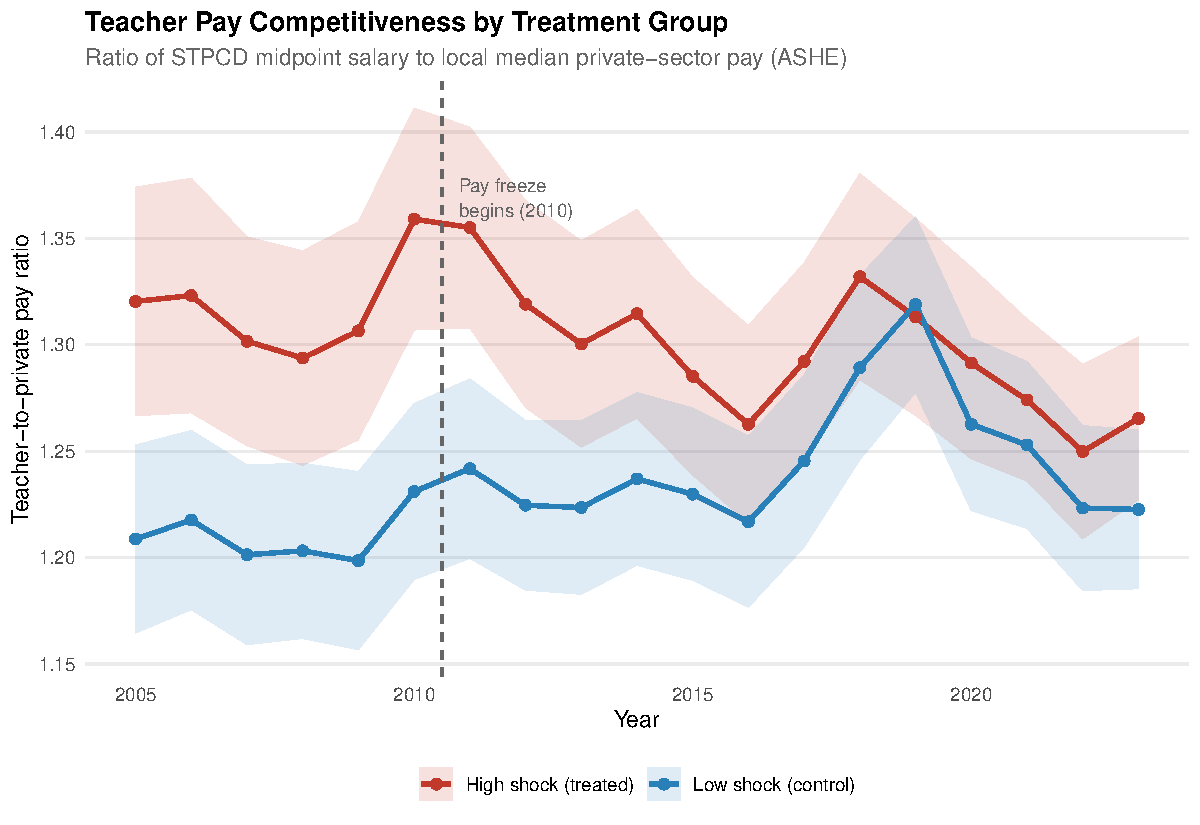
\includegraphics[width=0.85\textwidth]{figures/fig1_competitiveness_trends.pdf}
\caption{Teacher Pay Competitiveness by Treatment Group, 2005--2023}
\label{fig:trends}
\par\vspace{2pt}\noindent\small{\textit{Notes:} Mean ratio of STPCD midpoint teacher salary to ASHE local median private-sector annual pay, by treatment group. Shaded bands show 95\% confidence intervals. Dashed vertical line marks the start of the pay freeze (2010). Treatment defined as bottom quartile of the 2010--2019 competitiveness \textit{change} ($\Delta R_j$). Treated LAs start with higher absolute ratios (because private wages are lower in these areas) but experience the largest \textit{decline} in competitiveness over the austerity period---hence the convergence visible in the figure.}
\end{figure}

\subsection{Dose-Response Relationship}

\Cref{fig:dose} shows the scatter plot of LA-level competitiveness change against mean post-austerity Attainment~8, with a fitted OLS line. The positive slope indicates that areas with larger competitiveness \textit{improvements} (or smaller declines) had higher achievement. The relationship is driven by the extremes of the distribution: LAs with the most negative competitiveness changes cluster at lower achievement levels.

\begin{figure}[H]
\centering

\includegraphics[width=0.85\textwidth]{figures/fig5_dose_response.pdf}
\caption{Teacher Pay Competitiveness Change and Student Achievement}
\label{fig:dose}
\par\vspace{2pt}\noindent\small{\textit{Notes:} Each point is a local authority. Horizontal axis: change in competitiveness ratio between 2010 and 2019. Vertical axis: mean Attainment~8 score averaged over 2021/22--2023/24. Dashed line is OLS fit. Red = treated (Q1); blue = control (Q2--Q4).}
\end{figure}

\subsection{Panel Two-Way Fixed Effects}

As an additional specification, I estimate two-way fixed effects regressions at the LA-by-year level for the post-COVID sample (2021/22--2023/24), exploiting within-LA year-to-year variation in the competitiveness ratio:
\begin{equation}
\text{Att8}_{jt} = \alpha_j + \gamma_t + \beta R_{jt} + \varepsilon_{jt}
\end{equation}
where $\alpha_j$ are LA fixed effects and $\gamma_t$ are year fixed effects. Note that the regressor $R_{jt}$ is the \textit{level} of the competitiveness ratio in year $t$, while the cross-sectional specifications use the \textit{change} $\Delta R_j = R_{j,2019} - R_{j,2010}$. The panel sample comprises 141 LAs observed across three post-COVID academic years (2021/22--2023/24), but some LAs have missing Attainment~8 data in later years (141 in 2021/22, 137 in 2022/23, 134 in 2023/24), yielding an unbalanced panel with $N = 412$ LA-year observations. The coefficient $\beta$ on the competitiveness ratio level is $0.38$ (SE $= 0.88$, $p = 0.670$), which is positive (consistent with the cross-sectional results) but statistically insignificant. The null result reflects limited within-LA variation in competitiveness over the short post-COVID window: the STPCD midpoint changed modestly between 2021 and 2023, and ASHE wages exhibited year-to-year noise. The TWFE specification is therefore poorly powered to detect effects that the cross-sectional design captures through the accumulated 2010--2019 variation. The difference in coefficient magnitude between the TWFE ($0.38$ on $R_{jt}$) and the cross-sectional OLS ($7.73$ on $\Delta R_j$) reflects this change of regressor: a unit change in the \textit{level} of $R_{jt}$ within the short post-COVID window represents far less variation than a unit change in the decade-long \textit{difference} $\Delta R_j$.

I also estimate an interaction model with treatment status and year dummies. The treatment-by-year coefficients are $0.30$ ($p = 0.130$) for 2021 and $0.16$ ($p = 0.305$) for 2022, both positive but imprecise. These estimates should not be interpreted as event-study evidence, since treatment is defined over 2010--2019 and the ``event'' of the pay freeze has no sharp start date in the GCSE outcome data.

\subsection{Equity Analysis: FSM Achievement Gap}

The effect on the within-LA FSM achievement gap is null: $0.07$ points ($p = 0.913$). This suggests that the competitiveness shock affects overall achievement levels rather than exacerbating within-area inequality. If the mechanism operates through area-wide teacher supply constraints (fewer applicants to all schools), rather than selective sorting of teachers away from disadvantaged schools, this null is expected.

\subsection{Robustness and Sensitivity}\label{sec:robust}

\subsubsection{Alternative Treatment Definitions}

\Cref{tab:robust} presents results using alternative treatment cutoffs. The median split yields a near-zero estimate ($-0.08$, $p = 0.902$), consistent with the effect being concentrated in the tail of the competitiveness decline distribution. The tercile split is similarly null ($-0.17$, $p = 0.799$). When comparing only the extreme quartiles (top vs. bottom), the estimate increases to $-1.59$ ($p = 0.129$). This pattern suggests that moderate competitiveness declines have negligible effects; only the most severe erosion appears consequential.

\begin{table}[H]
\centering
\caption{Robustness: Alternative Treatment Definitions}
\label{tab:robust}
\begin{adjustbox}{max width=\textwidth}
\begin{threeparttable}
\begin{tabular}{lcccc}
\toprule
Specification & Estimate & Std. Error & $p$-value & $N$ \\
\midrule
Main (Q1 cutoff) & $-$0.85 & 0.71 & 0.233 & 141 \\
Median split & $-$0.08 & 0.61 & 0.902 & 141 \\
Tercile split & $-$0.17 & 0.68 & 0.799 & 141 \\
Extreme quartiles (Q1 vs. Q4) & $-$1.59 & 1.03 & 0.129 & 71 \\
\bottomrule
\end{tabular}
\begin{tablenotes}[flushleft]
\small
\item \textit{Notes:} All specifications include baseline private-sector pay and urban proxy as covariates. Heteroskedasticity-robust standard errors. Main specification uses bottom quartile as treatment. Extreme quartiles compare bottom and top quartile only, excluding middle 50\% ($N$ reduced accordingly).
\end{tablenotes}
\end{threeparttable}
\end{adjustbox}
\end{table}

\subsubsection{Propensity Score Sensitivity}

I re-estimate the DR-AIPW with alternative propensity score specifications. A simpler model using only baseline pay yields $-1.20$ ($p = 0.085$), nearly identical to the main logistic AIPW. A richer model adding region fixed effects to the propensity score yields $-0.45$ ($p = 0.648$), which is substantially attenuated. This sensitivity to the inclusion of region dummies reflects the strong geographic component of treatment assignment: London boroughs are overwhelmingly in the control group, while treated LAs are concentrated among Unitary and ``Other'' authorities.

\subsubsection{Leave-One-Region-Out}

The leave-one-region-out analysis reveals a key source of fragility. Excluding Unitary authorities (20 of 36 treated LAs) flips the sign to $+0.31$ ($p = 0.765$). Excluding Metropolitan boroughs strengthens the effect to $-1.40$ ($p = 0.120$). Excluding London boroughs or ``Other'' LAs produces intermediate estimates. This sensitivity indicates that the result is substantially driven by the comparison between Unitary treated LAs and London borough controls.

\subsubsection{Placebo Test}

The placebo test uses the 2005--2010 competitiveness change---which predates the austerity freeze---as a pseudo-treatment. If the conditional unconfoundedness assumption holds, this placebo should be null. The estimate is $-1.12$ ($p = 0.101$), which, while not conventionally significant, is uncomfortably large and of similar magnitude to the main result. This suggests that areas experiencing large competitiveness shifts in any period differ from other areas in ways that are imperfectly controlled by baseline pay and urban proxy alone. I interpret this as a warning that the main estimate may partially reflect persistent structural differences rather than the causal effect of the austerity pay squeeze.

\subsubsection{Omitted Variable Sensitivity}

Three complementary approaches assess sensitivity to unobserved confounders. First, Oster's (2019) coefficient stability test yields $\delta = 2.13$, meaning that unobservable confounders would need to be more than twice as important as the combined effect of baseline pay and urban proxy to fully explain the result. Under Oster's rule-of-thumb $R^2_{\max} = 2.2 \tilde{R}^2$, this exceeds the conventional threshold of $|\delta| > 1$.

Second, the E-value for the point estimate is 1.92, indicating that an unmeasured confounder would need to be associated with both treatment and outcome by a factor of approximately 1.9 to explain away the observed association. The E-value for the confidence interval bound is 1.00, meaning even modest confounding could move the interval to include zero.

Third, the sensemakr robustness value $RV_{q=1} = 0.167$ indicates that a confounder explaining 16.7 percent of the residual variance in both treatment and outcome would be sufficient to reduce the estimate to zero.

\subsubsection{Randomization Inference}

Fisher's exact randomization inference test yields a $p$-value of 0.236 based on 1,000 random permutations of the treatment assignment. This is larger than the parametric $p$-values, reflecting the limited effective sample size and suggesting that statistical significance of the OLS specification depends on distributional assumptions. \Cref{fig:perm} shows that the observed coefficient lies near the left tail but not far enough to reject at conventional levels under the randomization distribution.

\begin{figure}[H]
\centering
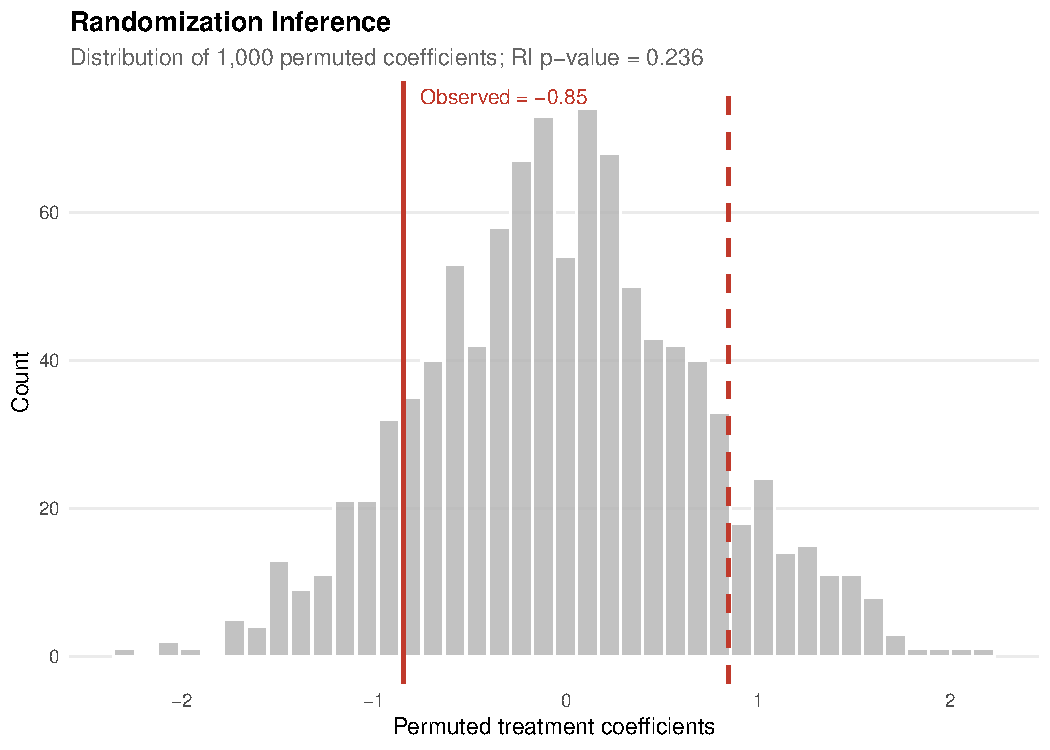
\includegraphics[width=0.85\textwidth]{figures/fig7_permutation_inference.pdf}
\caption{Randomization Inference: Distribution of Permuted Treatment Coefficients}
\label{fig:perm}
\par\vspace{2pt}\noindent\small{\textit{Notes:} Histogram of 1,000 permuted OLS coefficients from random reassignment of treatment labels. Solid red line: observed coefficient ($-0.85$). Dashed red line: mirror of observed coefficient. Two-sided $p$-value = 0.236.}
\end{figure}

\subsubsection{Year-by-Year Estimates}

Cross-sectional estimates by year are remarkably stable: $-0.83$ in 2018/19, $-0.73$ in 2021/22, $-0.79$ in 2022/23, and $-0.83$ in 2023/24. None is individually significant, but the consistency across years supports the interpretation of a persistent (rather than idiosyncratic) effect.

%=============================================================================
\section{Discussion}\label{sec:discussion}
%=============================================================================

\subsection{Interpretation}

The results provide suggestive evidence that the decade-long erosion of teacher pay competitiveness during England's austerity period had a modest negative effect on GCSE achievement. The preferred RF-AIPW estimate of $-1.12$ Attainment~8 points is statistically significant and robust to omitted variable diagnostics, but the evidence is not unambiguous. The OLS estimates with covariates are not significant, the randomization inference $p$-value is 0.236, and the placebo test raises concerns about structural differences between treated and control areas.

The effect magnitude is economically meaningful but not dramatic. A decline of 1.1 Attainment~8 points---roughly 2.4 percent of the mean---is small relative to the within-LA variation but non-trivial at the population level. Across 36 treated local authorities serving approximately 2 million students, even a modest effect on average achievement translates to thousands of students achieving one grade lower in one subject.

\subsection{Mechanisms}

I cannot directly observe the mechanisms through which competitiveness erosion affects achievement, as the School Workforce Census data on vacancies and retention are not available via the public API. However, the existing literature provides strong indirect evidence. \citet{sims2020teacher} documents that the pay squeeze reduced teacher applications by 11--13 percent per year relative to trend, with larger effects in competitive labour markets. \citet{allen2018teacher} show that teacher vacancy rates doubled between 2010 and 2018, with the worst shortages in STEM subjects and in London.

The null effect on the FSM achievement gap is consistent with an area-wide supply mechanism rather than within-school sorting. If all schools in a treated LA face a smaller and lower-quality applicant pool, achievement may fall across the board without differentially affecting disadvantaged schools. This contrasts with the US evidence \citep{clotfelter2008would}, where salary supplements targeted to high-poverty schools reduced turnover, implying that the distribution of teachers \textit{within} areas responds to pay signals.

\subsection{Limitations}

Several limitations temper the causal interpretation. First, the treatment is not exogenous. While the STPCD freeze is nationally imposed, the private-sector wage growth that drives treatment variation reflects local economic conditions that may independently affect education. The baseline controls are limited to pay, competitiveness, and a crude urban proxy; richer covariates---school spending, demographics, Ofsted ratings---would strengthen the design.

Second, the post-COVID timing introduces confounding. Areas that experienced larger competitiveness declines may also have experienced differential COVID impacts---through school closures, remote learning quality, or teacher absence---that affected the 2021--2024 GCSE cohorts independently of austerity-era teacher quality.

Third, the placebo test is not cleanly null. The 2005--2010 placebo estimate of $-1.12$ ($p = 0.101$) suggests that the cross-sectional relationship between competitiveness changes and achievement may partly reflect persistent area characteristics rather than a causal channel.

Fourth, the absence of pre-treatment LA-level GCSE data (the DfE API only provides LA-level data from 2018/19) precludes a difference-in-differences design or pre-trend analysis. This is the most significant limitation: without pre-treatment outcomes, I cannot verify that treated and control areas were on parallel achievement trajectories before the pay freeze.

\subsection{External Validity}

The results speak to the specific institutional setting of England's centralized teacher pay system during a period of fiscal austerity. The mechanism---uniform public-sector pay interacting with heterogeneous private-sector alternatives---is relevant to other countries with centralized pay scales (France, Germany, many developing countries) but less applicable to systems with local salary negotiations (many US states).

Several features of the English context limit generalizability. First, the UK private-sector labour market is relatively flexible, meaning that wage growth during the recovery period was genuinely driven by productivity and demand rather than collectively bargained increases. In countries with more rigid private-sector wages (e.g., France), the competitiveness mechanism would operate differently. Second, England's school system is highly accountable: Attainment~8 and Progress~8 are headline measures used in school inspections, league tables, and parent choice. This means teacher quality translates fairly directly into measured outcomes. In systems with less accountability or more heterogeneous assessment practices, the link might be weaker. Third, the magnitude of the pay freeze---nearly a decade of stagnation---is historically unusual. Shorter freezes or smaller real pay erosion might not generate detectable effects on a measure as noisy as LA-level GCSE averages.

\subsection{Policy Implications}

If the main estimate is taken at face value, a back-of-envelope calculation illustrates the aggregate cost. The 36 treated local authorities serve approximately 400,000 GCSE students per cohort. A decline of 1.1 Attainment~8 points per student corresponds to roughly 440,000 Attainment~8 points ``lost'' per year across the cohort. Using the conversion that one Attainment~8 point corresponds approximately to one GCSE grade in one subject, this is equivalent to 440,000 students each achieving one grade lower in one subject, or (more realistically) a smaller number of students experiencing larger deficits. The cumulative effect over the decade of austerity---given recruitment and retention lags---could be several times this annual figure.

These magnitudes should be compared against the fiscal savings from the pay freeze. Holding teacher pay at 2010 levels (in real terms) rather than allowing it to grow with CPI inflation saved the Exchequer approximately \textsterling{} 3--4 billion per year by 2019, considering the roughly 500,000 full-time equivalent teachers in England \citep{ifs2019teacher}. Whether the estimated achievement cost is ``worth'' these savings depends on one's valuation of a GCSE grade point---a question this paper cannot answer but the results can inform.

The geographic distribution of the effect is particularly relevant for equity. The areas experiencing the largest competitiveness declines are not affluent London suburbs (where private wages were already high) but rather Northern and Midlands areas where the teaching profession was historically competitive. The irony is that the nationally uniform freeze imposed the largest educational cost on areas that were already educationally disadvantaged---widening the gap between London and the rest of England rather than narrowing it.

%=============================================================================
\section{Conclusion}\label{sec:conclusion}
%=============================================================================

Between 2010 and 2019, England's public-sector pay freeze created substantial variation in teacher pay competitiveness across local authorities. Areas where private-sector wages grew fastest experienced the largest declines in the relative attractiveness of teaching. I find a negative association between competitiveness erosion and GCSE achievement: doubly robust estimates suggest a decline of approximately 1.1 Attainment~8 points in the most affected areas. This estimate is significant in-sample ($p = 0.037$) but not robust to cross-fitted inference or randomization-based tests, and the placebo test raises concerns about pre-existing differences.

The evidence is suggestive rather than definitive. The absence of pre-treatment outcome data prevents a difference-in-differences design; the placebo test raises concerns about baseline differences; and significance depends on the choice of estimator. These caveats are important for policy interpretation. Nonetheless, the finding aligns with a growing body of evidence that teacher pay matters for educational outcomes, not just for teacher supply \citep{hanushek2011economic, dolton2011if, hendricks2014relative}.

Three avenues for future research emerge from this analysis. First, the availability of school-level workforce data from the School Workforce Census---currently restricted to accredited researchers---would allow direct estimation of the recruitment and retention mechanisms linking pay competitiveness to teacher quality. Linking SWC data on vacancy rates, teacher experience distributions, and subject specialisms to school-level GCSE outcomes would provide a richer picture of the causal chain. Second, the recent recovery in teacher starting salaries (to \textsterling{} 30,000 by 2023) creates a mirror image of the austerity shock: studying whether achievement recovers in formerly squeezed areas would test the symmetry of the relationship. Third, extending the analysis to other public-sector professions facing similar pay dynamics---nurses, police officers, social workers---would test the generality of the ``uniform pay, heterogeneous markets'' mechanism.

The policy implications are straightforward in direction, if uncertain in magnitude. The 2022 STRB recommendation to raise starting salaries to \textsterling{} 30,000 was motivated by recruitment concerns. This paper suggests that the decade preceding that increase may have already imposed an achievement cost---one that fell disproportionately on areas where private-sector wage growth outpaced the frozen teacher pay scale. The lesson is not simply that teachers should be paid more, but that nationally uniform pay schedules, when frozen, interact with spatial labour market dynamics to create uneven educational consequences. The fiscal savings of the austerity pay freeze were clear and immediate; the educational costs, until now, remained hidden.

\section*{Acknowledgements}

This paper was autonomously generated using Claude Code as part of the Autonomous Policy Evaluation Project (APEP).

\noindent\textbf{Project Repository:} \url{https://github.com/SocialCatalystLab/ape-papers}

\noindent\textbf{Contributors:} @SocialCatalystLab

\noindent\textbf{First Contributor:} \url{https://github.com/SocialCatalystLab}

\label{apep_main_text_end}
\newpage
\bibliography{references}

\newpage
\appendix

%=============================================================================
\section{Data Appendix}\label{app:data}
%=============================================================================

\subsection{ASHE Earnings Data}

The Annual Survey of Hours and Earnings (ASHE) data are accessed via the NOMIS web API at \url{https://www.nomisweb.co.uk/api/v01/}. The specific dataset is NM\_99\_1 (ASHE Table 8: Place of Work). I extract median annual gross pay (item=2, pay=7, measures=20100) for all employees (sex=7) at the local authority district level (geography=TYPE464) for each year from 2005 to 2023.

ASHE reports at the lower-tier district level (E07 codes), which does not match the upper-tier education authority level (E10 county codes). I construct a manual lookup table mapping each of 165 districts to their parent county, then compute the county-level median private-sector pay as the unweighted mean of constituent district medians. This approach assumes that districts within a county are broadly similar; population-weighted aggregation would be preferable but district-level population data are not included in the ASHE extract.

The final dataset contains 2,680 LA-year observations across 146 unique education authorities and 19 years.

\subsection{Key Stage 4 Data}

KS4 results are accessed from the Department for Education Explore Education Statistics API (dataset ID: b3e19901-5d2b-b676-bb4c-e60937d74725). The dataset includes Attainment~8, Progress~8, English and Maths basics pass rates, and counts of pupils and schools, disaggregated by geography level, sex, FSM status, and other breakdowns.

I filter to geographic\_level = ``Local authority,'' breakdown\_topic = ``Total'' (or ``FSM status'' for the equity analysis), and sex = ``Total.'' The time\_period variable is a six-digit code (e.g., 202324); I extract the academic year as the first four digits. Data are available at the LA level from 2018/19 onward; earlier years provide only national and regional aggregates.

\subsection{STPCD Pay Scales}

Teacher pay scale reference points are hand-coded from published STPCD documents available on GOV.UK. The M1 (starting salary) and M6 (top of main pay range) for the Rest of England pay band are recorded for each year from 2005 to 2023. The midpoint salary used in the competitiveness ratio is $(M1 + M6) / 2$.

\begin{table}[H]
\centering
\caption{STPCD Main Pay Range, Rest of England, 2005--2023}
\label{tab:stpcd}
\begin{adjustbox}{max width=\textwidth}
\begin{threeparttable}
\begin{tabular}{ccccc}
\toprule
Year & M1 (\textsterling{}) & M6 (\textsterling{}) & Midpoint (\textsterling{}) & Nominal growth (\%) \\
\midrule
2005 & 19,161 & 28,005 & 23,583 & --- \\
2006 & 19,641 & 28,707 & 24,174 & 2.5 \\
2007 & 20,133 & 29,427 & 24,780 & 2.5 \\
2008 & 20,627 & 30,148 & 25,388 & 2.5 \\
2009 & 21,102 & 30,842 & 25,972 & 2.3 \\
2010 & 21,588 & 31,552 & 26,570 & 2.3 \\
2011 & 21,588 & 31,552 & 26,570 & 0.0 \\
2012 & 21,588 & 31,552 & 26,570 & 0.0 \\
2013 & 21,804 & 31,868 & 26,836 & 1.0 \\
2014 & 22,023 & 32,187 & 27,105 & 1.0 \\
2015 & 22,244 & 32,509 & 27,377 & 1.0 \\
2016 & 22,467 & 32,831 & 27,649 & 1.0 \\
2017 & 23,720 & 33,824 & 28,772 & 4.1 \\
2018 & 24,373 & 35,971 & 30,172 & 4.9 \\
2019 & 25,714 & 38,174 & 31,944 & 5.9 \\
2020 & 25,714 & 38,174 & 31,944 & 0.0 \\
2021 & 25,714 & 38,174 & 31,944 & 0.0 \\
2022 & 28,000 & 38,810 & 33,405 & 4.6 \\
2023 & 30,000 & 41,333 & 35,667 & 6.8 \\
\bottomrule
\end{tabular}
\begin{tablenotes}[flushleft]
\small
\item \textit{Notes:} M1 is the minimum starting salary on the main pay range. M6 is the maximum. Midpoint is $(M1 + M6)/2$. Nominal growth is the year-on-year percentage change in the midpoint. Source: Published STPCD documents, GOV.UK.
\end{tablenotes}
\end{threeparttable}
\end{adjustbox}
\end{table}

\subsection{District-to-County Aggregation}

For the 21 two-tier counties in England, I construct a lookup table mapping lower-tier district codes (E07) to their parent county codes (E10). The mapping covers 165 districts. County-level ASHE earnings are computed as the unweighted mean of constituent district medians.

%=============================================================================
\section{Identification Appendix}\label{app:id}
%=============================================================================

\subsection{Balance Diagnostics}

\Cref{tab:balance} reports standardized mean differences (SMDs) and $t$-test $p$-values for baseline characteristics. The SMDs for baseline pay ($-0.654$) and baseline competitiveness ($0.656$) exceed the conventional threshold of 0.25, confirming substantial imbalance. The DR-AIPW estimator addresses this through reweighting, but the large imbalance limits the effective sample size and increases sensitivity to model specification.

\begin{table}[H]
\centering
\caption{Baseline Balance (2010 Characteristics)}
\label{tab:balance}
\begin{adjustbox}{max width=\textwidth}
\begin{threeparttable}
\begin{tabular}{lccccc}
\toprule
Variable & Treated & Control & Difference & SMD & $p$-value \\
\midrule
Baseline private-sector pay (\textsterling{}) & 19,829 & 22,186 & $-$2,357 & $-$0.654 & $<0.001$ \\
Baseline competitiveness ratio & 1.36 & 1.23 & 0.13 & 0.656 & $<0.001$ \\
Urban proxy & 0.31 & 0.54 & $-$0.23 & $-$0.466 & 0.012 \\
\bottomrule
\end{tabular}
\begin{tablenotes}[flushleft]
\small
\item \textit{Notes:} SMD is the standardized mean difference computed as $({\bar{X}}_T - {\bar{X}}_C) / \sigma_{\text{pooled}}$. Urban proxy equals one if baseline pay exceeds the sample median. $p$-values from two-sample $t$-tests.
\end{tablenotes}
\end{threeparttable}
\end{adjustbox}
\end{table}

The region distribution also differs: treated LAs are 56\% Unitary authorities and only 6\% London boroughs, while controls are 30\% Unitary and 29\% London boroughs. This geographic concentration of treatment is a key source of identification fragility.

\subsection{Sensitivity Contour Plot}

\Cref{fig:sensitivity} shows the Cinelli and Hazlett (2020) sensitivity contour plot for the continuous treatment specification. The benchmark covariate (baseline pay) is marked with a triangle. The plot shows the combinations of confounder strength (as fractions of the benchmark's explanatory power) that would be needed to reduce the estimate to zero or to move the confidence interval to include zero.

\begin{figure}[H]
\centering
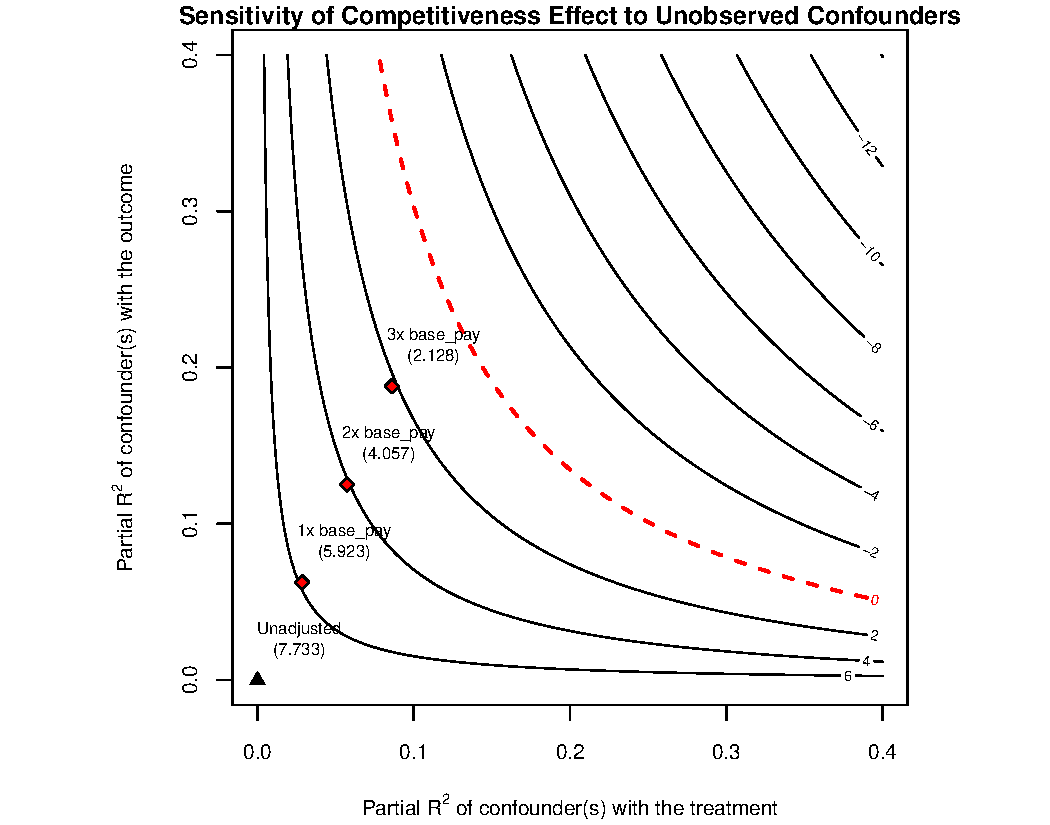
\includegraphics[width=0.85\textwidth]{figures/fig8_sensitivity_contour.pdf}
\caption{Sensitivity of Competitiveness Effect to Unobserved Confounders}
\label{fig:sensitivity}
\par\vspace{2pt}\noindent\small{\textit{Notes:} Contour plot from the sensemakr package \citep{cinelli2020making}. Axes represent the partial $R^2$ of a hypothetical unobserved confounder with treatment (horizontal) and outcome (vertical). The red line shows combinations that would reduce the estimate to zero. Triangle marks the benchmark covariate (baseline pay). The robustness value $RV_{q=1} = 0.167$ indicates that a confounder explaining 16.7\% of residual variance in both dimensions would nullify the result.}
\end{figure}

%=============================================================================
\section{Robustness Appendix}\label{app:robust}
%=============================================================================

\subsection{National Pay Trends}

\Cref{fig:paytrends} displays the national trends in teacher and private-sector pay. The austerity freeze is clearly visible: teacher pay flatlines between 2010 and 2016 while private-sector pay continues to grow. The divergence is most pronounced between 2014 and 2019.

\begin{figure}[H]
\centering
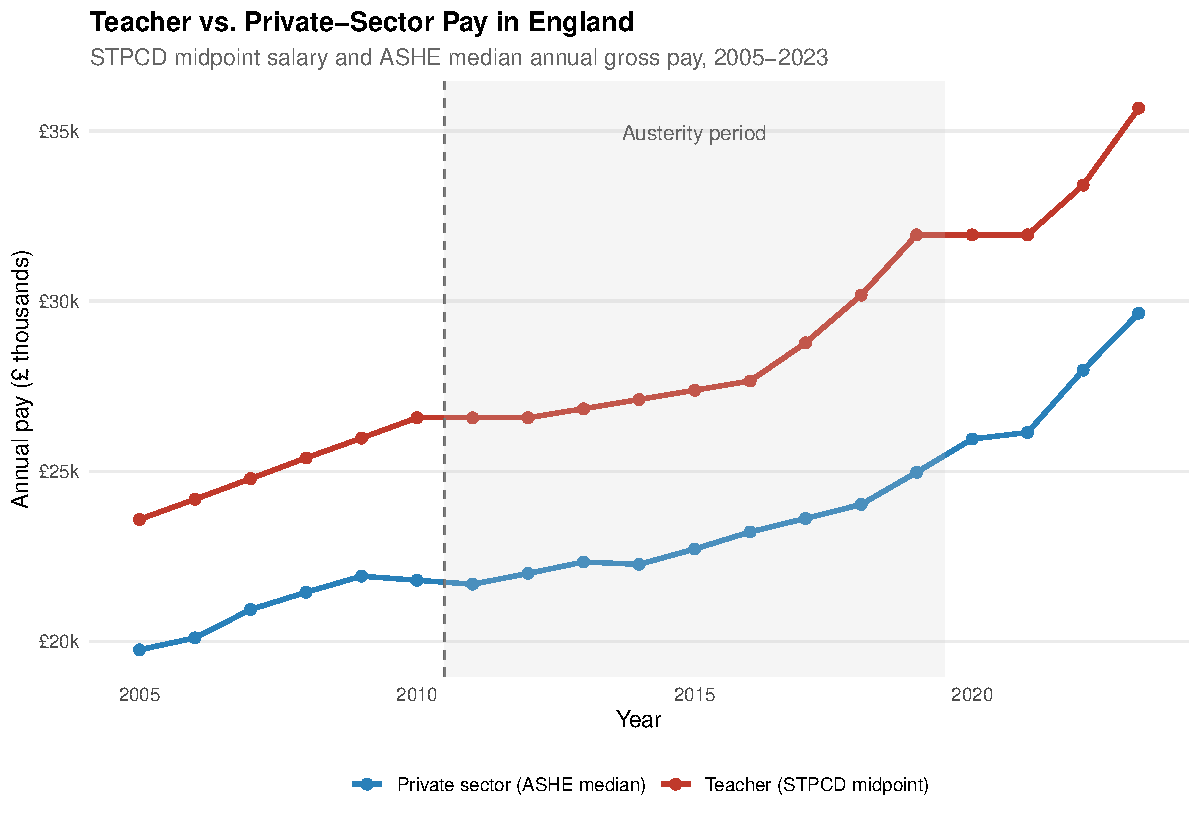
\includegraphics[width=0.85\textwidth]{figures/fig2_pay_trends.pdf}
\caption{Teacher vs. Private-Sector Pay in England, 2005--2023}
\label{fig:paytrends}
\par\vspace{2pt}\noindent\small{\textit{Notes:} STPCD midpoint salary (Rest of England) and national average ASHE median annual gross pay. Shaded area denotes the austerity period (2010--2019).}
\end{figure}

\subsection{STPCD Component Trends}

\Cref{fig:stpcd_components} decomposes the STPCD into its constituent points. The M1 starting salary was frozen at \textsterling{} 21,588 from 2010 to 2012, then increased by 1\% annually through 2016. The larger increases from 2017 onward were concentrated at M1 (reflecting government efforts to address recruitment), while M6 grew more slowly.

\begin{figure}[H]
\centering
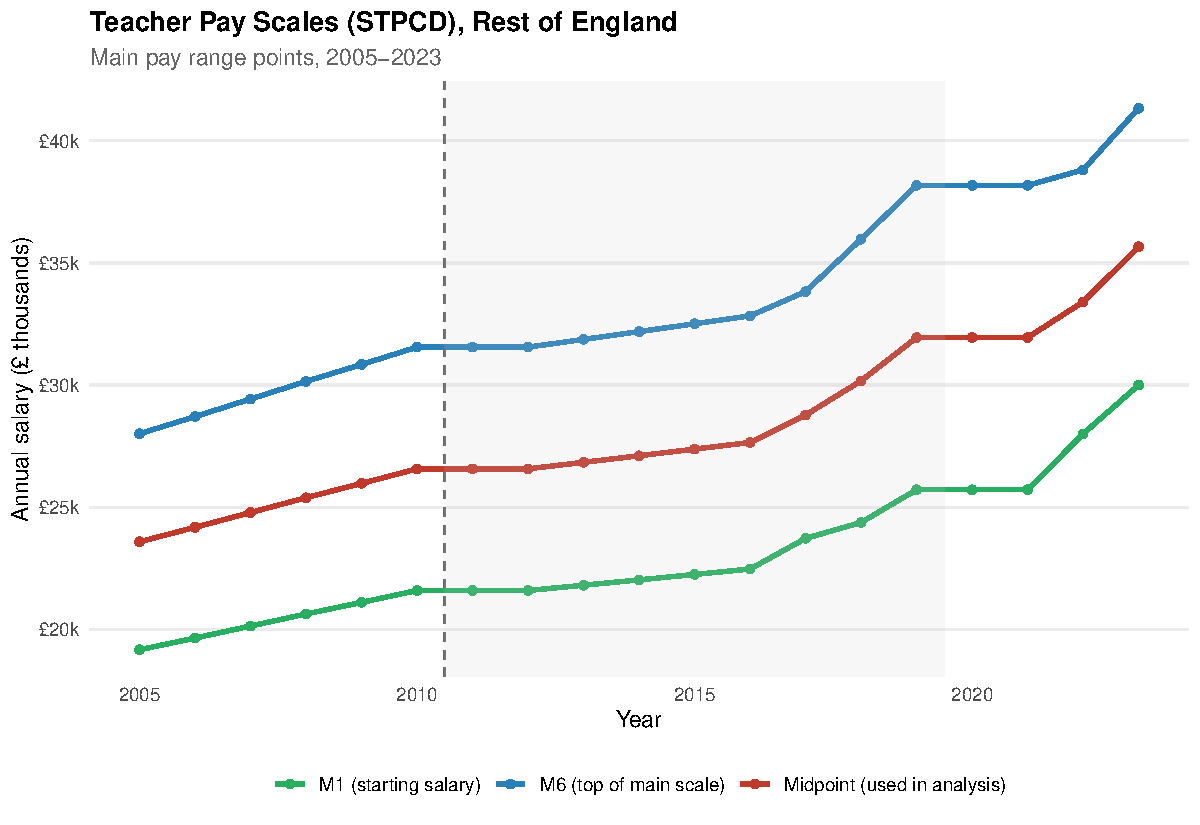
\includegraphics[width=0.85\textwidth]{figures/fig9_stpcd_components.pdf}
\caption{STPCD Pay Scale Components, Rest of England}
\label{fig:stpcd_components}
\par\vspace{2pt}\noindent\small{\textit{Notes:} M1 = starting salary, M6 = top of main pay range, Midpoint = $(M1+M6)/2$.}
\end{figure}

\subsection{Treatment Assignment Distribution}

\Cref{fig:treat_dist} shows the distribution of the 2010--2019 competitiveness change across local authorities, with the bottom-quartile threshold marked. Most LAs experienced a decline in competitiveness (the distribution is left-skewed), but the magnitude varies substantially. The treated group includes LAs with declines of 0.08--0.30 in the competitiveness ratio.

\begin{figure}[H]
\centering
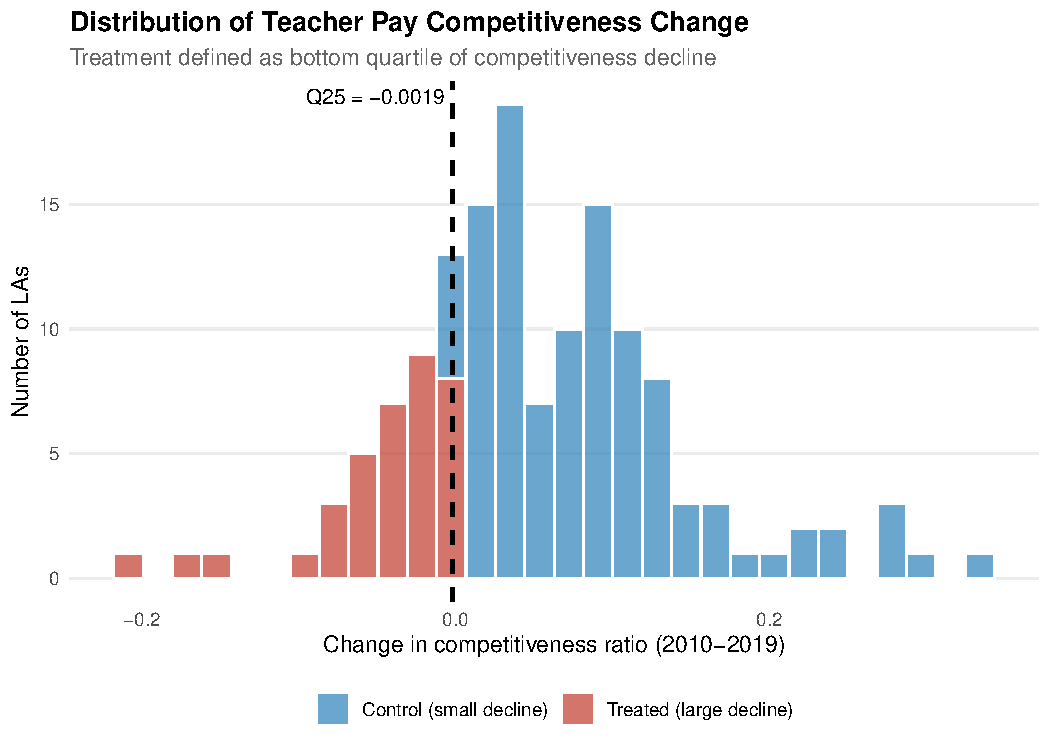
\includegraphics[width=0.85\textwidth]{figures/fig4_treatment_assignment.pdf}
\caption{Distribution of Teacher Pay Competitiveness Change, 2010--2019}
\label{fig:treat_dist}
\par\vspace{2pt}\noindent\small{\textit{Notes:} Histogram of $\Delta R_j = R_{j,2019} - R_{j,2010}$ across 141 local authorities in the analysis sample. Red bars: treated (Q1, largest decline). Blue bars: control (Q2--Q4). Dashed line: Q1 threshold.}
\end{figure}

\subsection{Year-by-Year Treatment Effects}

\Cref{fig:yearly} displays cross-sectional treatment effect estimates by year. The estimates are remarkably consistent across years, ranging from $-0.73$ to $-0.83$ Attainment~8 points. None is individually significant at conventional levels, but the stability suggests a persistent relationship rather than year-specific confounding.

\begin{figure}[H]
\centering

\includegraphics[width=0.85\textwidth]{figures/fig6_yearly_effects.pdf}
\caption{Treatment Effect by Year}
\label{fig:yearly}
\par\vspace{2pt}\noindent\small{\textit{Notes:} OLS coefficient on the binary treatment indicator from year-specific cross-sectional regressions including baseline pay and urban proxy as controls. Error bars show 95\% confidence intervals with heteroskedasticity-robust standard errors.}
\end{figure}

\subsection{Full Sensitivity Summary}

\begin{table}[H]
\centering
\caption{Sensitivity Analysis Summary}
\label{tab:sensitivity}
\begin{adjustbox}{max width=\textwidth}
\begin{threeparttable}
\begin{tabular}{lcc}
\toprule
Test & Value & Interpretation \\
\midrule
Placebo (2005--2010 change) & $-$1.12 ($p = 0.101$) & Non-trivial; raises concern \\
Randomization inference & $p = 0.236$ & Not significant under permutation \\
Oster $\delta$ ($R^2_{\max} = 0.59$) & 2.13 & Robust ($|\delta| > 1$) \\
E-value (point estimate) & 1.92 & Moderate confounder needed \\
E-value (CI bound) & 1.00 & Minimal confounder to include zero \\
Sensemakr $RV_{q=1}$ & 0.167 & 16.7\% residual variance to nullify \\
Sensemakr $RV_{q\alpha}$ & 0.014 & 1.4\% to move CI to include zero \\
\bottomrule
\end{tabular}
\begin{tablenotes}[flushleft]
\small
\item \textit{Notes:} Oster $\delta$ computed under the rule-of-thumb $R^2_{\max} = 2.2 \tilde{R}^2$. E-values computed following \citet{vanderweele2017sensitivity}. Sensemakr robustness values computed following \citet{cinelli2020making} with baseline pay as benchmark covariate.
\end{tablenotes}
\end{threeparttable}
\end{adjustbox}
\end{table}

%=============================================================================
\section{Heterogeneity Appendix}\label{app:hetero}
%=============================================================================

\subsection{Region-Specific Estimates}

The leave-one-region-out analysis reveals significant heterogeneity by LA type:

\begin{table}[H]
\centering
\caption{Leave-One-Region-Out Estimates}
\label{tab:loo}
\begin{adjustbox}{max width=\textwidth}
\begin{threeparttable}
\begin{tabular}{lcccc}
\toprule
Excluded Region & Estimate & Std. Error & $p$-value & $N$ \\
\midrule
None (full sample) & $-$0.85 & 0.71 & 0.233 & 141 \\
Unitary & $+$0.31 & 1.03 & 0.765 & 89 \\
Metropolitan & $-$1.40 & 0.90 & 0.120 & 105 \\
London Borough & $-$0.62 & 0.57 & 0.284 & 109 \\
Other & $-$1.22 & 0.83 & 0.143 & 120 \\
\bottomrule
\end{tabular}
\begin{tablenotes}[flushleft]
\small
\item \textit{Notes:} OLS with baseline pay and urban proxy controls. Heteroskedasticity-robust standard errors. Each row excludes all LAs of the indicated type. $N$ varies as regions are excluded.
\end{tablenotes}
\end{threeparttable}
\end{adjustbox}
\end{table}

Excluding Unitary authorities eliminates and reverses the treatment effect, confirming that the result is driven by comparisons involving this LA type. This is not surprising given that 20 of 36 treated LAs are unitary authorities, but it limits the external validity of the finding.

\end{document}
